\documentclass[a4paper]{article}

\usepackage[english]{babel}
\usepackage[utf8x]{inputenc}
\usepackage{amsmath}
% \usepackage{amssymb}
\usepackage{float}
% \usepackage{graphicx}
\usepackage[authoryear]{natbib}
\usepackage{hyperref}
% \usepackage{authblk}
\usepackage[margin=1in]{geometry}
\usepackage{pgfplots}
\pgfplotsset{compat=1.12}
\PrerenderUnicode{ü}

\title{Mapintel Project Report}
\author{David Silva, Fernando Bação}
\date{\today}

\begin{document}

\maketitle

\begin{abstract}
	Briefly summarize your previous work, goals and objectives, what you have accomplished, and future work. (100 words max) If you have a question, please use the help menu (''?'') on the top bar to search for help or ask us a question.
\end{abstract}

\section*{Introduction}
% Introducing the topic: https://www.investopedia.com/ask/answers/022615/what-effect-has-globalization-had-international-investments.asp
Globalization has an increasingly important impact on businesses and economies around the world. It has influenced international investing, increased communication and awareness of business opportunities, and led to more connections among financial markets. Even though this has opened a lot of new opportunities, it has also substantially increased competitiveness among businesses worldwide. This creates the necessity for companies to closely monitor and understand the external business environment in which they are inserted.

Competitive Intelligence (CI) is a system of environmental scanning that involves the collection and analysis of information with the objective to achieve competitive advantage. According to \citet{brod1999}, "Companies with competitive intelligence programs have better knowledge of their markets, better cross-functional relationships between their business units and a greater ability to develop proactive competitive strategies." A survey made to CI professionals in \citet{marin2004} revealed that the most common sources of CI are news providers, corporate websites and trade publications and that it can be obtained from a wide variety of channels such as employees, clients and suppliers. CI has a fundamental role in helping businesses remain competitive, influencing a wide range of decision-making areas, and leading to substantial improvements such as the increase of revenue, new products or services, cost savings/avoidance, time savings, profit increases, and achievement of financial goals \citep{calof2017}.

% Need to better understand how CI is used by AICEP
The Trade \& Investment Portuguese Agency (AICEP) "is a government business entity, focused in encouraging the best foreign companies to invest in Portugal and contribute to the success of Portuguese companies abroad in their internationalization processes or export activities", making AICEP a major contributor to the economic development and job creation in Portugal. CI is a key component of AICEP's activity, as it is used to keep track of external corporate, economic, technological, and science-related events. An important part of the CI process at AICEP surrounds the daily reading of news articles from multiple sources and topics to scan/understand the changes in the environment, detect possible investment opportunities, and ultimately generate a competitive advantage. 

Despite the high availability of such data, it is hard for the analysts to get a clear picture of the current environment state as the process of sifting through news articles is highly ineffective and can easily lead to missed opportunities and incomplete views of the current panorama. To address the information overload felt by AICEP's analysts, we propose a CI system that enables the exploration and search of up-to-date news articles from a myriad of national and international news sources. This tool allows its users to interactively explore and discover information through the use of data visualization and information retrieval techniques. Furthermore, we use Natural Language Processing (NLP) models to represent the articles as vectors that reliably encode their semantics, while spatially organizing the data. The system helps the user to quickly gain knowledge about the current state of the environment and easily satisfy any information need that might emerge through the exploration.

% In this project we look to answer the research question: \textbf{What aspects does a document exploration system require to extract meaningful information from a continuous flow of text documents?} We use Natural Language Processing and Machine Learning algorithms to represent and analyze the text documents, particularly we use document embedding models such as Paragraph Vector \citep{Le2014} to represent the documents in a vector space which encodes the semantics of each document and Self-Organizing Maps (SOM) \citep{Kohonen1982} to explore and visualize the different segments of documents in that space.
% In this project we look to answer the specific question: How can a visual exploration tool be produced to extract information from a continuous flow of text documents? / What components should a news exploration system have to enable efficient information retrieval tasks?

\section*{Literature Review}
% This paragraph talks about IR 
Information Retrieval (IR) is the process of "finding material of an unstructured nature that satisfies an information need from within large collections" \citep[p.~1]{schutze2008}. This process is done daily by millions of persons for a wide variety of reasons. The most common interaction we have with IR is through web search engines, which allows a person to make ad hoc queries and receive relevant results. The IR process requires that the user defines a specific information need and can express it through a given query. This may result in a problem as oftentimes the need cannot be framed as a query. This happens mainly when the user wants to go through a set of documents without any particular objective but to assess them and understand which information they contain, both as a whole and individually. We denominate this process as \textit{Document Exploration}. Document exploration usually involves a user reading through a large document collection and progressively gaining knowledge of the topics mentioned by each document. This is exactly what AICEP analysts do in order to gather intelligence, and it will be one of the focus of our work. 

% This paragraphs talks about the Vector Space Model
The Vector Space Model (VSM) \citep[p.~120-126]{schutze2008} consists of representing a set of documents as vectors in a common vector space, while also allowing free-text queries to be represented in this same space. The fundamental assumption of VSM is that similar documents will be placed close together in the vector space, whereas dissimilar documents will be far away. This model is essential for dealing with large document collections as it ranks the documents matching a query, providing only the most relevant results. This is contrasted by the Boolean Retrieval model \citep[p.~1-18]{schutze2008}, which given a Boolean expression of terms, can return a number of matching documents superior to the one a human user could possibly sift through. The VSM ranks each document $d$ in decreasing order of their cosine similarity with a query $q$: 
\begin{equation}
	cosine(q,d) = \frac{\overrightarrow{V}(q).\overrightarrow{V}(d)}{|\overrightarrow{V}(q)||\overrightarrow{V}(d)|}
\end{equation}

, where $\overrightarrow{V}(q)$ corresponds to the query vector and $\overrightarrow{V}(d)$ corresponds to the document vector. VSM can be easily extended to clustering and classification applications as these require text input to be represented as fixed-length vectors. 

% This paragraph talks about document embedding literature. Classical: BOW, TF-IDF | Topic Modeling: LSI, pLSI, LDA | Neural Embeddings: Word2vec, GloVe, Doc2vec | BERT-based Embeddings: BERT, SBERT
One of the most common fixed-length representations of text is bag-of-words \citep{harris1954}, due to its simplicity, efficiency and often surprising accuracy. Term frequency-inverse document-frequency (TF-IDF) \citep{jones1972} is another representation which tries to correct some problems of bag-of-words by not giving the same importance to every feature. Both these models have two main disadvantages: the word order is lost, which means different sentences can have the same representation as long as they have the same word frequencies e.g. "I like maths but not physics" has the same representation as "I like physics but not maths", and semantics are ignored, which results in representations that don't account for the actual meaning of the sentence. To solve the later issue and in particular, the inability of these representations to deal with synonymy (the same information can be described using different terms) and polysemy (a term can express several distinct meanings depending on its context), \citet{deerwester1990} proposes the Latent Semantic Indexing (LSI). LSI consists in applying singular-value decomposition to construct a low-rank approximation of the term-document matrix, thus mapping both terms and documents into a low k-dimensional orthogonal semantic space that preserves, to some extent, the relative distances between vectors in the original space. Once this mapping is obtained, new documents and queries can be represented in the semantic space and similarities can be computed as in the VSM. The representations provided achieve great savings in both storage and query time. Intuitively, LSI is able to capture the semantic structure in the data because it is forced to squeeze the terms/ documents down to a low k-dimensional space bringing together terms with similar co-occurrences. Therefore, the documents (and queries) are no longer represented by terms, but by the underlying concepts referred by the terms. 

Despite the good empirical results in IR \citep{dumais1988, berry1995}, LSI does not provide a mathematical explanation for its effectiveness, leaving us with unanswered questions regarding the extent to which it captures the semantic structure of a corpus \citep{papadimitriou2000}. \citet{hofmann1999} addresses this issue by proposing Probabilistic LSI (pLSI), a statistical latent variable model that defines a proper generative model for general co-occurrence data. pLSI models each word $w \in W = \{w_1, ..., w_M\}$ in a document $d \in D = \{d_1, ..., d_N\}$ as a sample from a document-specific word distribution $P(w|d)$ that is characterized as a mixture model \citep[p.~337-380]{murphy2012} of $K$ latent factors $Z = \{z_1, ..., z_K\}$ with mixture weights $\theta = P(z|d)$, where $z \in Z$. More concretely, pLSI is defined as a joint probability model:

\begin{subequations}
	\begin{align}
		P(d,w) & = P(d)P(w|d), where \\
		P(w|d) & = \sum_{k=1}^K P(w|z_k)P(z_k|d)
	\end{align}
\end{subequations}

The pLSI model posits that observation pairs $(d, w)$ are generated independently i.e. "bag-of-words" assumption, and that documents and words are conditionally independent given a topic $z$. The model parameters, $P(d)$, $P(w|z)$ and $P(z|d)$ are estimated by maximizing the log-likelihood function:

\begin{equation}
	\mathcal{L} = \sum_{n=1}^N \sum_{m=1}^M n(d_n,w_m)logP(d_n,w_m) 
\end{equation}

, where $n(d,w)$ gives the term frequency of $w$ in $d$. The optimization algorithm used is a variation of the Expectation Maximization (EM) \citep[p.~348-369]{murphy2012}. pLSI represents each document in the training set with the mixture weights $P(z|d)$ and thus queries (and new documents) need to be folded-in by computing $P(z|q)$, where $q$ denotes a query made by the user, using EM iteration. Then, the low dimensional representations are used by VSM to rank each document according to a query.

Latent Dirichlet Allocation (LDA) \citep{blei2003} is a generative probabilistic model of a corpus. Contrarily to pLSI, LDA can naturally assign probabilities to previously unseen document, thus being a well-defined generative model of documents. Also, in pLSI the number of parameters grows linearly with the size of the corpus, which makes it prone to overfitting, whereas in LDA the number of parameters is independent of it. Both these improvements are achieved by treating the topic mixture weights $\theta$ as a $K$-dimensional Dirichlet hidden random variable rather than a $K\times N$ matrix of parameters, where the mixture weights are linked to the training documents $D$. According to LDA, a document $d$ can be generated as follows:

% Check equations below and if z should have also index m or not.
\begin{subequations}
	\begin{align}
		P(d|\alpha,\beta) & = \int P(\theta|\alpha)\left(\prod_{m=1}^M P(w_m|\theta,\beta)\right) d\theta, where \\
		P(w_m|\theta,\beta) & = \sum_{k=1}^K P(w_m|z_k,\beta)P(z_k|\theta)
	\end{align}
\end{subequations}

, where $\theta \sim Dir(\alpha)$, $\alpha$ is a $K$-vector with components $\alpha_i >$ 0 and $\beta$ is a $K\times V$ matrix, where $\beta_{ij}=P(w^j=1|z^i=1)$ and $V$ is the vocabulary size. $\theta$ can be seen as a document-specific probability distribution over the topics, $\alpha$ is the Dirichlet distribution parameter and each row of $\beta$ gives a topic-specific probability distribution over the vocabulary. By assuming that documents in a corpus are independent, we can obtain the probability of a corpus $D$:

\begin{equation}
	P(D|\alpha,\beta) = \prod_{n=1}^N P(d_n|\alpha, \beta)
\end{equation}

LDA is a three-level hierarchical Bayesian model, thus the generation of corpus can be divided into three stages: sample the corpus-level parameter $\alpha$ and $\beta$ once, sample the document-level variables $\theta_n$ once per document and sample the word-level variables $z_nm$ and $w_nm$ once for each word in each document.
% This section about the LDA and pLSI needs to be refactored to standardize the notation of the formulas! The best way I see to do it is by writing a Notation and terminology section like in the LDA paper.

% Doc2Vec section here
While the probabilistic approaches mentioned above can represent a document as a vector of topic probabilities, thus being frequently referred as topic modeling, there is a more recent and equally common alternative to represent documents as a dense fixed-length vector that utilizes a neural network architecture and an unsupervised task to learn the representations. This approach is usually called neural embedding modeling and is able to produce document embeddings (i.e. document vector representations) that account for word order and capture the semantics of the words, two of the main issues of the classical BOW model. A prime example of this approach is the Paragraph vector model \citep{le2014} (or Doc2Vec model), an unsupervised algorithm that learns both word and document vectors by minimizing the error of predicting the next word in a paragraph (a variable-length piece of text) given the paragraph and previous word vectors. The neural network is parameterized by the word and document vectors which are trained using stochastic gradient descent and backpropagation. This architecture is inspired by the CBOW (Continuous BOW) and Skip-gram word embedding models in \citet{mikolov2013}.

% Transformer, Attention, BERT, SBERT section here
With the recent advent of the Transformer architecture, significant improvements were made in several tasks related with Natural Language Processing (NLP) \citet{vaswani2017}. This new architecture is based solely on attention mechanisms, providing parallelization capabilities and significant improvements in training time. Also, the Transformer can more easily learn long-range relationships between terms in the input sequence than the pre-existing Recurrent Neural Network (RNN) \citep{} and Convolutional Neural Network (CNN) \citep{} architectures. The Bidirectional Encoder Representation from Transformers (BERT) is a Transformer based pre-trained language model that can be easily fine-tuned to obtain state-of-the-art level performance for multiple NLP tasks \citep{devlin2019}. BERT differences itself from the other pre-trained language models by utilizing a "masked language model" pre-training task that uses both left and right context to predict randomly masked terms from the input sequence. In addition, the model is also pre-trained on a "next sentence prediction" task that jointly pre-trains text-pair representations.

Despite the versatility and good performance obtained by BERT in various sentence classification and sentence-pair regression tasks, there isn't a natural way to obtain an independent sentence embedding since by design BERT takes as input two sentences separated by a special token and outputs the sentence token representations. Most importantly, "finding the most similar pair in a collection of 10,000 sentences requires about 50 million inference computations (~65 hours) with BERT" \citep{reimers2019}, making this an inadequate approach for obtaining document embeddings to be used for semantic textual similarity (STS) and in particular for IR. Sentence-BERT or SBERT \citep{reimers2019} solves this issue by using a siamese network structure that adds a pooling layer to the output of a pre-trained BERT model. By passing a single sentence as input to BERT and then aggregating its outputs with the pooling layer, we can derive a fixed sized sentence embedding, reducing to around 5 seconds the time taken to perform the task described above. The weights are fine-tuned with Natural Language Inference (NLI) data, resulting in embeddings that can capture the semantics of each sentence and can be used with VSM for IR related tasks.

% Paragraph about Top2Vec or BERTopic

% This paragraph talks about visualizing high-dimensional spaces (U-matrix, t-SNE and UMAP)
We already discussed how we can embed documents in a semantically coherent vector space. Furthermore, we also mentioned how we can utilize the document vectors to retrieve relevant results to a given user query. Now we focus on the approaches for representing the local and global patters within the document collection in a visual interface that facilitates the document exploration task. t-SNE \citep{vandermaaten2008} is arguably the most well known and one of the best performing algorithms for visualizing high-dimensional data in a 2 or 3 dimensional map. t-SNE builds this map by minimizing the Kullback-Leibler divergence between the joint probability distribution of the neighborhood of each pair of observations in the high-dimensional space and the joint probability distribution of the neighborhood of each pair of observations in the map. The minimization is solved with the use of gradient descent. UMAP \citep{mcinnes2020} is a more recent algorithm for visualizing high-dimensional data. Contrarily to t-SNE, it provides a "general purpose dimension reduction technique that is grounded in strong mathematical foundations" \citep{mcinnes2020} related to Riemannian geometry and algebraic topology. The output map is obtained by minimizing the cross-entropy between the topological representations of the high-dimensional space and the map. The minimization is too solved with gradient descent. In practical terms, UMAP compares favorably to t-SNE \citep{mcinnes2020} by achieving an equivalent or better map quality, by being more stable over different runs and under sub-sampling, by significantly reducing the time required to produce the output map, by supporting significantly larger data set sizes and by imposing no restriction on embedding dimensions.

Another frequently used technique for visualizing and organizing high-dimensional data is Self-Organizing Map (SOM) \citep{Kohonen1982}. SOM works by fitting a grid of units to the data points in a high-dimensional input space. The fitting is done through an iterative process where each data point is allocated to the nearest unit in the input space, the BMU (best matching unit), then the BMU together with its neighbor units (defined according to a neighborhood function) are moved in the direction of the data point. This process is repeated until we reach a given stopping criterion. Besides having an input space representation, each unit has an output space position. This output space consists of an arrangement of units in a 2 dimensional grid. This output space is what offers SOM its visualization capabilities by representing some properties of the input space. By grayscale coding each unit in the 2D output space with the distance in the input space between itself and its neighboring units we obtain a U-matrix \citep{ultsch1993}. This visualization allows us to see regions of the input space that are close together or isolated giving us a sense of the topology of the original input space.

\section*{Related work}
% Introduction: The introduction should clearly establish the focus and purpose of the literature review.
% Body: Summarize and synthesize, Analyze and interpret, Critically evaluate, Write in well-structured paragraphs
% Conclusion: summarize the key findings you have taken from the literature and emphasize their significance.
Our work is inspired by previous applications related to visual analytics, SOM and exploration of large collection of documents.

\citet{ji2019} proposes a system for visual exploration of neural document embeddings to gain insights into the underlying embedding space and to promote the utilization in prevalent IR applications. t-SNE is used to project the high-dimensional data onto a 2D surface. This technique is able to capture both local and global structure from the high-dimensional data in an efficient and reliable way. In this work, the documents are embedded using the Paragraph Vector model. The system visualizes neural document embeddings as a configurable document map and enables guidance and reasoning, facilitates to explore the neural embedding space, identifies salient neural dimensions (semantic features) per task and domain interest and supports advisable feature selection (semantic analysis) along with instant visual feedback to promote IR performance. Overall, the system provides users with insights and confidence in neural document embeddings given their black-box nature.

\citet{lafia2019} uses SOM and Latent Dirichlet Allocation (LDA) to convey the relatedness of research themes in a multidisciplinary university library. Documents are represented as random mixtures over latent topics, where each topic is characterized by a distribution over words. That said, each document is embedded in a vector space of N dimensions, corresponding to the number of topics selected. SOM produces a landscape for exploring the topic space and provides users with an overview of the document collection and the ability to navigate (discover items of interest), change the level of detail, select individual documents and discover relationships between documents.

\citet{kaski1998} presents the WEBSOM - a system that organizes a textual document collection using a SOM-based graphical map display that provides an overview of the collection and facilitates interactive browsing. \citet{kohonen2013} revisits the topic and provides some enhancements. Here, the documents are represented with a TF-IDF weighting and a random projection is used to reduce the dimensionality of the vector space, while preserving the similarity structure between documents. A SOM is constructed and each document is mapped into the node that best represents it. This provides exploring, searching and filtering capabilities. For example, when a node in the map is clicked, the titles of the corresponding documents and eventually some additional information such as descriptive words are presented. Also, the map is described by an automatic annotation procedure explained in \citet{lagus1999}, which helps to understand the semantics encoded in each map region. The user can also perform queries either using a set of keywords or a descriptive sentence. The query is then mapped into the reduced vector space and matched with the most similar documents and/or nodes. A zooming feature is also present which allows the user to explore specific regions of the map with finer detail.

\citet{henriques2012} proposes the GeoSOM suite, a tool for geographic knowledge discovery using SOM. This tool is designed to integrate geographic information and aspatial variables in order to assist the geographic analyst's objectives and needs. The tool provides several dynamically linked views of the data consisting of a geographic map, an u-matrix, component plate plots, hit-map plots, parallel coordinate plots, boxplots and histograms. These views and their connection allows for an interactive exploration of the data.
% Discuss what is already known about your research area. Connect your objectives with what is already known and explain what additional contribution you intend to make. Make sure to add APA formatted in-text citations like this \citep{tennekes_first_1972}. If you mention the author(s) in your sentence, you can simply give the year of publication. For example, \citet{tennekes_first_1972} wrote an excellent book on turbulence. You can find it online \href{https://newcatalog.library.cornell.edu/catalog/8325020}{here}. As you are reviewing literature, you may find a need to write equations. A graphical tool for generating \LaTeX \ equations can be found \href{www.hostmath.com}{here}. Part of writing equations can include referring to obscure symbols and Greek letters. A tool for doing that visually (by drawing) can be found \href{http://detexify.kirelabs.org/classify.html}{here}.

% Write about Sara Lafia paper
\citep{lafia2021a} proposes a method for modeling and mapping topics from bibliometric data and build a web application based on this method. They also perform a user evaluation of the topic map. The map produced allows users to read a body of research "at a distance", while providing multiple levels of detail of the topics that represent the documents. They also incorporate a time dimension, allowing users to understand the evolution of the topics over time. They compare both non-negative matrix factorization (NMF) \citep{lee1999} and LDA for discovering the underlying topics in the data and obtaining vector representations of the documents. For visualizing these documents, they compare both t-SNE and UMAP. The best performing configuration uses NMF with t-SNE. To allow for different detail levels, the authors produce two maps: a coarse map of 9 topics that gives a general overview of the topics within the data and a detailed map of 36 topics that captures more specific research themes. The web application consists of an interactive dashboard that allows users to explore the map of documents.

\section*{Methods}
The methodology adopted in this project can be summarized by Figure \ref{Methodology}. First, we set up a data collection process to automatically absorb the continuous flow of news articles, then some pre-processing was applied to the data to make it usable by the embedding models and improve the quality of the produced document vectors. A SOM was applied to build a two-dimensional grid that is able to represent the multi-dimensional input space and therefore, the properties and relationships of the articles. Finally, a document exploration interface was built to provide the user the ability to explore and query the articles. The code developed for the project can be accessed at \href{https://github.com/DavidSilva98/mapintel_project}{github.com/DavidSilva98/mapintel\_project}.
\begin{figure}[H]
	\centering
	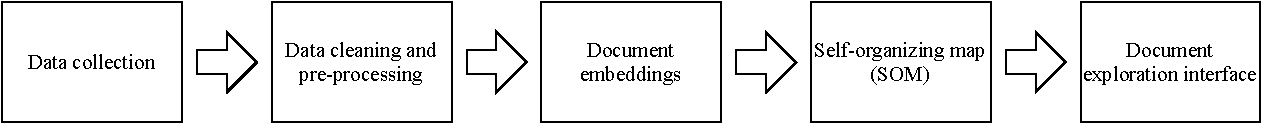
\includegraphics[scale=0.7]{./figures/methodology}
	\caption{Methodology}
	\label{Methodology}
\end{figure}
\subsection*{Data Collection}
In this project we decided to focus on how NLP and particularly sentence embeddings could help in organizing, exploring and retrieving text documents. Since the objective is to explore news articles, we used a REST API \footnote{\href{https://newsapi.org/}{newsapi.org}} to continuously retrieve English articles from multiple international sources several times a day. The API calls are performed through the AWS Lambda service \footnote{A serverless compute service that lets you run code without provisioning or managing servers} and the articles, as well as their metadata, are stored using the MongoDB Atlas cloud database service \footnote{A fully-managed cloud database service}. One particularly useful feature of the metadata is the category of the article. This can be one of the following: business, entertainment, general, health, science, sports or technology. It is important to note that the API we are using imposes some limitations that affect the data collection such as the articles being provided with 1 hour delay, having a maximum of 100 requests per day and the content of the article being truncated to 200 characters. We also developed a simple Optical Character Recognition (OCR) pipeline using the Tesseract OCR engine \footnote{\href{https://github.com/tesseract-ocr/tesseract}{github.com/tesseract-ocr/tesseract}}. The purpose of this pipeline was to integrate internal documents from AICEP in our application, however we haven't focused on these documents so far.


\subsection*{Data Cleaning and Pre-processing}
After loading the document corpus from the database, we concatenated the title, description and content fields in order to obtain longer and more informative documents. We proceed to clean the documents by removing non-textual patterns such as URLs and HTML tags and by removing non-English articles which are still present despite the filter applied previously. We split the document corpus into train and test set to allow for downstream unbiased performance assessments. A pre-process pipeline is applied on both corpora \footnote{Note: the pipeline is fitted only on the train set to avoid data leakage} to reduce the dimensionality of the vocabulary. The pipeline consists of removing stop words (very frequent words that are irrelevant), lowering the letter's case, removing accents and punctuation, applying stemming \footnote{Term normalization process that removes the morphological and inflectional endings from words} and removing words that appear in just one document or in more than 90\% of the documents.

\subsection*{Document Embeddings}
Once the corpus is pre-processed, we encoded each document as a single vector of information. Here we used several approaches and compared them using a standardized evaluation design. As a baseline we used a Bag-of-Words (BOW) approach \citep{harris1954}, which represents each document as a token histogram of the top 10000 most frequent tokens. We also used a Term Frequency - Inverse Document-Frequency (TF-IDF) approach \citep{jones1972} which tries to adjust for the fact that some words appear more frequently in general by offsetting each token frequency with the number of documents that contain the token. In these 10000 tokens, we included n-grams containing one to three words so word order information could be included in the embedding. We also used the proposed models by \citet{le2014}, namely the Distributed Memory Model of Paragraph Vectors (PV-DM) and the Distributed Bag of Words version of Paragraph Vector (PV-DBOW), to learn continuous distributed fixed-length vector representations from variable-length pieces of text. These models are trained on the task of predicting words in a paragraph by looking at the context of the target word, which is encoded in the words and paragraph vectors. These vectors are the parameters of the model and are adjusted using stochastic gradient descent and backpropagation. One of the disadvantages of these methods is that to infer the embeddings of new documents, the model needs to train them which can be a problem when dealing with user queries.

\subsubsection*{Model Evaluation}
To evaluate the quality of each approach, we used the corresponding embeddings and categories of each document in various tasks, similarly to some of the ones in \citet{conneau2018}. One of the approaches was training a logistic regression model using the embedding vectors of the train corpus to predict the article category. The accuracy of the classifier on the test corpus was used to evaluate the embeddings as the model is kept constant over the different approaches. We realized that, even though the model is kept constant, we cannot control for the interactions between each feature set and the logistic regression, which means the scores obtained don't completely isolate the embeddings performance. For this reason, a second task was proposed which consisted in classifying whether each unique test document pair belonged to the same category, based solely on their cosine similarity. The cosine similarities were converted to a range between 0 and 1 using the min-max transformation and the average binary cross-entropy over all unique pairs of documents was obtained. We also looked at the t-SNE projections of the embeddings to visualize how well they captured the semantics of the documents. Our hope was that if some semantic properties were captured, the embedding vectors would have been grouped by their categories. In the results section we will analyze how the different embedding models produced different evaluations.

\subsection*{Self-Organizing Map}
After comparing the several embedding models, the SOM model was applied on the train embeddings of the best performing model using a fork of the SOMPY package \citep{moosavi2014}. The grid is composed of regular hexagons as they are "visually much more illustrative and accurate, and are recommended" \citep{kohonen2013}. Also, we selected the lengths of the horizontal and vertical dimensions of the grid to comply with the relation of the two largest principal components, while providing enough nodes to adequately represent the details and clusters of the input space. The oblong regular arrays have the advantage over the square ones of guaranteeing faster and safer convergence in learning. The nodes were initialized as a regular, two-dimensional sequence of vectors taken along a hyperplane spanned by the two largest principal components of the input space, providing faster ordering and convergence \citep{kohonen2001}. Finally, we relied on the minimization of the quantization error (the mean distance of every data point to the corresponding best-matching unit) to select the remaining hyper-parameters of the model.

\subsection*{Document Exploration Interface}
We extracted the fitted codebook matrix and we utilized it to build a U-matrix \citep{ultsch1993} to visualize the structures of the high-dimensional input space. By adding an interactive component to this visualization, we were able to encode several details and information within each unit of the matrix such as the distance from its neighbor units, the number of observations allocated to it and also some aggregated information from these observations. We also used the approach in \citet{lagus1999} to characterize regions of the U-matrix by optimal positioning of descriptive keywords. These words function as landmarks i.e. navigational cues that help in maintaining a sense of location during the exploration of the map. Finally, we integrated the remaining components of the interface such as the search bar, a pane to preview the articles retrieved by the query and some more dynamic components to facilitate the user interaction.

% Explain the techniques you have used to acquire additional data and insights. Reserve fine detail for the Manual at the end of the report, but use this section to give an overview with enough detail for the reader to understand your Results and Analysis. Describe your apparatus, and have a justification for every decision you made and every parameter you chose in the design of the apparatus. Be especially careful to detail the conditions your experiments were conducted under, as this information is especially important for interpreting your results

% Below, some example sections are given. Sectioning the report is meant to keep similar information together.  Continue making sections as necessary, or delete sections if you do not need them. Feel free to add subsubsections to further delineate the information. For example, under the Experimental Apparatus section below, the EStaRS team might consider having sections such as "Filter Design" and "Filter Fabrication".

% \subsection*{Experimental Apparatus}
% Explain your apparatus setup using enough detail such that future teams can recreate your apparatus. Make sure to explain why you built it this way.
% \begin{itemize}
% 	\item Design (calculations, constraints)
% 	\item Schematic (label parts)
% 	\item Image (from lab; label parts)
% 	\item Materials (dimensions, materials)
% 	\item Complications in construction
% 	\item If already constructed: write a brief summary of important constraints, include any revisions to apparatus, also reference the prior report where construction is described
% \end{itemize}

% \subsection*{Procedure }
% Discuss your experimental procedure. How did you run your experiment? What were you testing? What were the values of relevant parameters?

\section* {Results}
Present an observation (results), then explain what happened (analysis).  Each paragraph should focus on one aspect of your results. In that same paragraph, you should interpret that result.
In other words, there should not be two distinct paragraphs, but instead one paragraph containing one result and the interpretation and analysis of this result. Here are some guiding questions for results and analysis:

When describing your results, present your data, using the guidelines below:
\begin{itemize}
	\item What happened? What did you find?
	\item Show your experimental data in a professional way. Refer to \href{https://confluence.cornell.edu/display/AGUACLARA/Grammar+Guidelines+for+Reports}{Grammar Guidelines for Reports} for details on formatting. Be sure to reference figures before they appear in your paper (see Figure \ref{Frog}). Be sure to do the same for tables (see Table \ref{Table}). For a good tool for making tables, go to \href{www.tablesgenerator.com}{tablesgenerator.com}.
\end{itemize}

\begin{figure}[H]
	\centering
	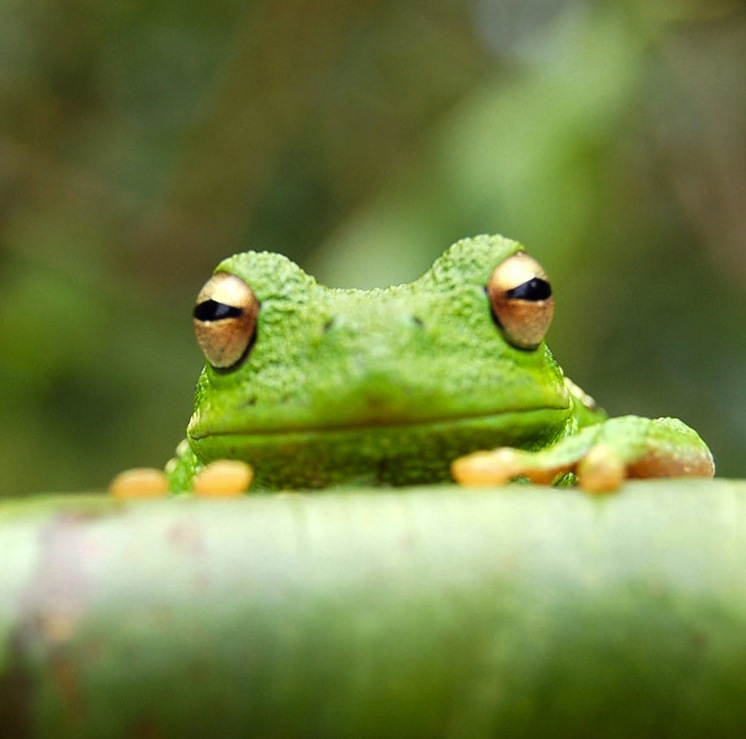
\includegraphics[scale=0.1]{./figures/frog}
	\caption{Captions go beneath figures.}
	\label{Frog}
\end{figure}

\begin{table}[H]
	\centering
	\caption{Captions go above tables.}
	\begin{tabular}{| l | c | c |}
		\hline
		Parameter          & Symbol   & Value                 \\ \hline
		Residence Time     & $\theta$ & 90 s                  \\ \hline
		Hydraulic Gradient & $G$      & 500 $\mathrm{s^{-1}}$ \\
		\hline
	\end{tabular}
	\label{Table}
\end{table}

After describing a particular result, within a paragraph, go on to connect your work to fundamental physics/chemistry/statics/fluid mechanics, or whatever field is appropriate. Analyze your results and compare with theoretical expectations; or, if you have not yet done the experiments, describe your expectations based on established knowledge. Include implications of your results. How will your results influence the design of AguaClara plants? If possible provide clear recommendations for design changes that should be adopted. Show your experimental data in a professional way using the following guidelines:
\begin{itemize}
	\item Why did you get those results/data?
	\item Did these results line up with expectations?
	\item What went wrong?
	\item If the data do not support your hypothesis, is there another hypothesis that describes your new data?
\end{itemize}

\section*{Discussion}
Study comparison with other studies. What were the limitations?

\section*{Conclusions}
Explain what you have learned and how that influences your next steps. Why does what you discovered matter to AguaClara?
Make sure that you defend your conclusions. (this is conclusions, not opinions!)

\section*{Future Work}
% Describe your plan of action for the next several weeks of research. Detail the next steps for this team. How can AguaClara use what you discovered for future projects? Your suggestions for challenges for future teams are most welcome. Should research in this area continue?
For implementing the query feature of the system, the query is embedded in the same space of the news article corpus and the distance with each SOM unit is computed. The query is then matched with the closest SOM unit and the documents allocated to that unit are retrieved. This approach is fast since there are many fewer units than documents. The unit's documents are ranked by computing the distance between them and the query. The search quality is expected to not decrease significantly as long as the Mean Quantization Error (MQE) (i.e. the mean euclidean distance each input vector to its BMU) remains low.

We plan to provide a zooming capability on the SOM U-matrix so the user can explore specific regions of the map in detail. There are two ways we have been discussing on how to implement this: one possibility would be to allow the user to select a specific unit or group of units on the map and then provide a projection of the underlying documents using either t-SNE \citep{vandermaaten2008} or UMAP \citep{mcinnes2020}; a second possibility would be to allow the user to digitally zoom in on the U-matrix, just like it is done in \citet{kaski1998}. An appealing attribute of this option is the preservation of the landmark labels, which are updated according to the zooming of the map.

There's also some discussion on how to integrate release date information on the article's representation. This would allow the documents to be organized not only according to their semantics but also according to their release date. This could also improve the query results as the users are most likely interested on current information. Another feature related to release date would be to relate documents in a time line, allowing a specific subject to be tracked through time. 

We would also like to improve the data collection pipeline since we are relying directly on NewsAPI free subscription which has some limitations already described. This would require a substantial effort since web scrapping would most likely be the necessary solution. This approach would provide us with the full article content and would allow us to collect articles as soon as they are released. Multilingual articles could also be collected and integrated into the system by using multilingual embeddings models such as \citet{conneau2019}.

Some more ideas to explore consist on: build a single or multi article summary feature, to provide a brief resume of the content of a specific article or of a specific SOM unit (collection of articles); add a news article feed based on individual user viewing history. If we plan to expand the application to multiple users, an implicit feedback collaborative filtering \citep{hu2008} approach could be used.

Some research on understanding the document embedding dimensions' would also be interesting as these usually present a correlation structure which captures the latent semantical topics of the document collection as seen in \citet{ji2019}. This would provide the user with the necessary confidence on the neural document embeddings that is lacking because of the black-box nature of these models.

\bibliographystyle{apalike}
\bibliography{bibliography}
\end{document}